%% SECTION HEADER /////////////////////////////////////////////////////////////////////////////////////
\section{Chosen \ac{shm} techniques using \acp{pzt}}
\label{sec:techniques}

%% SECTION CONTENT ////////////////////////////////////////////////////////////////////////////////////

\subsection{Guided waves based techniques}


\Acp{gw} are mechanical vibrations being a superposition of shear and longitudinal waves propagating in a bounded elastic medium, e.g., bars, beams, rods, plates and shells. 
Guided waves are multi-modal and dispersive, i.e. more than one mode travels simultaneously through the medium with the phase velocity depending on the frequency.
Fig.~\ref{fig:dispersion} shows an example of dispersion curves generated by Dispersion Calculator~\cite{huber2021dispersion} software tool for a 1 mm thick \ac{cfrp} plate up to 2000 kHz generated.
\Ac{a0} and \ac{s0}, considering the distribution of particle displacements on the upper and lower free surface relative to a central surface, are observed for low frequencies.
The mode shapes are pictured in Fig.~\ref{fig:mode_shape}, with the \ac{s0} particle displacements being dominant in-plane, while the \ac{a0} is dominated by out-of-plane.
Moreover, higher harmonic modes appear over the cut-off frequency, as shown in Fig.\ref{fig:dispersion}.
\begin{figure}
	%	\begin{center}
	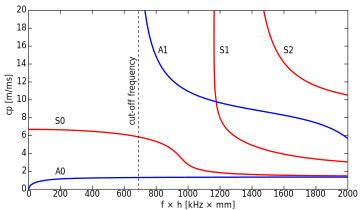
\includegraphics[width=1\linewidth]{Intro/dispersion}
	%	\end{center}
	\caption{Dispersion diagram for a 1 mm \ac{cfrp} plate (adopted from Dispersion Calculator~\cite{huber2021dispersion}). Red and blue solid curves represent symmetric, and asymmetric modes, respectively, black dashed line indicates cut-off frequency for higher modes.}
	\label{fig:dispersion}
\end{figure}
\begin{figure}
	%	\begin{center}
	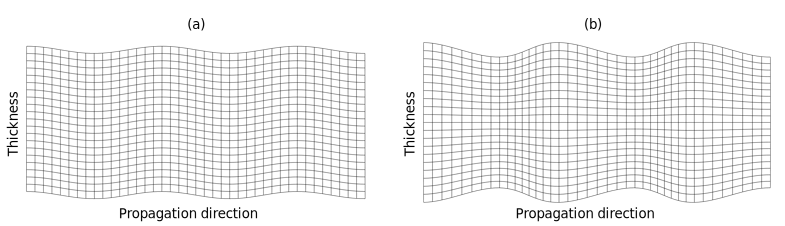
\includegraphics[width=1\linewidth]{Intro/mode_shape}
	%	\end{center}
	\caption{Mode shape of the \textbf{(a)} \ac{a0} and \textbf{(b)} \ac{s0} at 100 kHz for \(\phi=0^{\circ}\) in 2 mm composite plate (exported from Dispersion Calculator~\cite{huber2021dispersion}).}
	\label{fig:mode_shape}
\end{figure}

Detection schemes based on \acp{gw} exploit reflection, attenuation, and mode conversion when the propagating wave encounter a discontinuity in the structure. \cite{alleyne1992interaction}.
According to the one of the axiom of the \ac{shm} 
Thus, this technique is efficient to detect various types of defects, such as delamination \cite{sohn2011delamination,tian2015delamination}, adhesive disbonds \cite{rucka2018damage,balasubramaniam2021ultrasonic}, corrosion changes \cite{alleyne1995long,lowe1998defect}, cracks \cite{tua2004detection,lu2006crack,zima2020detection} and failures occurring in \acp{hsc} \cite{mustapha2011assessment, sikdar2016guided, sikdar2016ultrasonic,radzienski2016assessment, yu2019core}.
Many techniques based on \ac{gw} propagation have been developed for damage detection and localization.
A pitch-catch technique \cite{ihn2008pitch, sikdar2017structural} uses a pair of detached sensors, one of which excites and the other receives a signal.
The signal will be attenuated if it encounters a defect along its path.
In the case of the pulse-echo technique \cite{guo1993interaction, kudela2008damage}, there is one sensor that excites the wave and at the same time registers possible echo from the damage.
The damage localization can be determined if the wave speed is known and the time of flight is measured.
The radar principles were utilized in a phased array technique for plate inspection \cite{giurgiutiu2004embedded, ostachowicz2008elastic, kudela2018structural}.
The technique uses an array of transducers, each excited with an appropriate time offset, to focus all the waves at a single grid point of the area to be inspected.
A damage map is determined once the signals are obtained and processed for the entire grid.
Fink proposed a different approach, developing what he called a time-reversal mirror \cite{fink1992time}.
In this method, the wave propagates from one sensor to another, and then after time-reversal and dispersion compensation, the wave is re-emitted to the origin sensor.
The resulting signal will be a mirror image of the forcing signal only if the wave does not encounter damage along the way \cite{park2007time, eremin2016analytically}.

The \acp{pzt} can be used mutually as actuator-receiver pairs or as a single actuator with other types of devices, e.g. \ac{sldv}, \ac{fbg} sensors.
The \acp{pzt} generate high forces with broadband frequency, so methods based on \ac{gw} can detect various damage types of different sizes in a large inspected area.
Moreover, specific algorithms do not require a baseline model, and the method implementation is economically efficient.

\subsection{Electromechanical impedance methods}
The \ac{emi} spectroscopy is also an effective and powerful technique in \ac{shm} for real-time structural damage assessment \cite{park2003overview}.
The basis of this method is the influence of the mechanical impedance of the inspected host structure on the electrical impedance of the \ac{pzt} attached to the structure.
Assuming that the mechanical property of the sensor remains unchanged over the monitoring period, any changes in measurements of the electrical impedance can be considered a difference in the structure stiffness, which in turn can indicate that a defect has occurred.

Fundamentals of the \ac{emi} method were introduced by Liang et al. \cite{liang1994impedance}.
An analytical model of \ac{pzt} actuator bonded to one end of a single degree of freedom mass-spring-damper system was presented in this pioneering work.
In the early papers the authors adopted quasi-static sensor approximation until  Giurgiutiu and Zagrai \cite{giurgiutiu2000characterization} derived an expression where the dynamics of a sensor was incorporated.
The dynamics of single \ac{pzt} with various boundary condition (free, clamped and elastically constrained) and sensor attached to a beam were considered.
Further investigation \cite{zagrai2001electro, giurgiutiu2005damage} for the sensor bonded to the host structures was performed.
Damage detection is realized by comparing the state of the structure with the reference state using overall statistical damage indices, e.g.the \ac{rmsd}, the \ac{mapd}, \ac{ccd} and \ac{pnn}.
Malinowski et al. \cite{malinowski2014characterisation, malinowski2015use} investigated the effects of \ac{emi} changes related to the state of the adhesive layer between two composite plates.
The technique has been used to evaluate weak bonds due to inadequate adhesive curing temperature, release agent and moisture contamination. This type of damage is not detectable using the method based on \ac{gw} propagation.
Experimental testing was conducted on weakened samples and compared with a reference.
The \ac{rms} of both the conductance in range 3-5 MHz, and the first thickness resonant frequency shift were considered for bond-line assessment.

An and Sohn \cite{an2012integrated} propsed a new damage detection technique which combines advantages of \ac{emi} and \ac{gw}.
In the method, measured admittance characteristic is separated into two parts: active and passive.
\Ac{di} is a weighted sum of two indicators obtained from \ac{gw} signal and active admittance.
Because passive impedance is only sensitive to temperature variation, it is used for temperature compensation on both mentioned signals.
Instead of two \ac{di}, \cite{sevillano2016damage} proposed more integrated \ac{di} based on electromechanical power dissipation of the \ac{pzt} sensor.

The \ac{emi} technique can detect damage, such as delamination or cracks, but is also sensitive to changes, such as weak bonds, which the \ac{gw} method is ineffective at detecting. However, \ac{emi} is a local method that analyzes the structure within the sensor area, and its results vary widely depending on external conditions.

%\subsection{Modal analysis techniques}